\section{Processamento de Linguagem Natural}
\label{s.nlp}

\begin{frame}{Processamento de Linguagem Natural}
	\begin{itemize}
		\justifying	
		\item Quaisquer formas de comunicação, escrita ou verbal, carregam vastas quantias de informação, as quais podem ser utilizadas para \textbf{prever} o comportamento humano;
		\\~\\
		\item Tais informações \textbf{não} são \textbf{triviais} de serem analisadas, pois cada ser humano possui características inerentes à sua forma de comunicação.
	\end{itemize}
\end{frame}

\begin{frame}
	\begin{figure}[!ht]
		\centering
		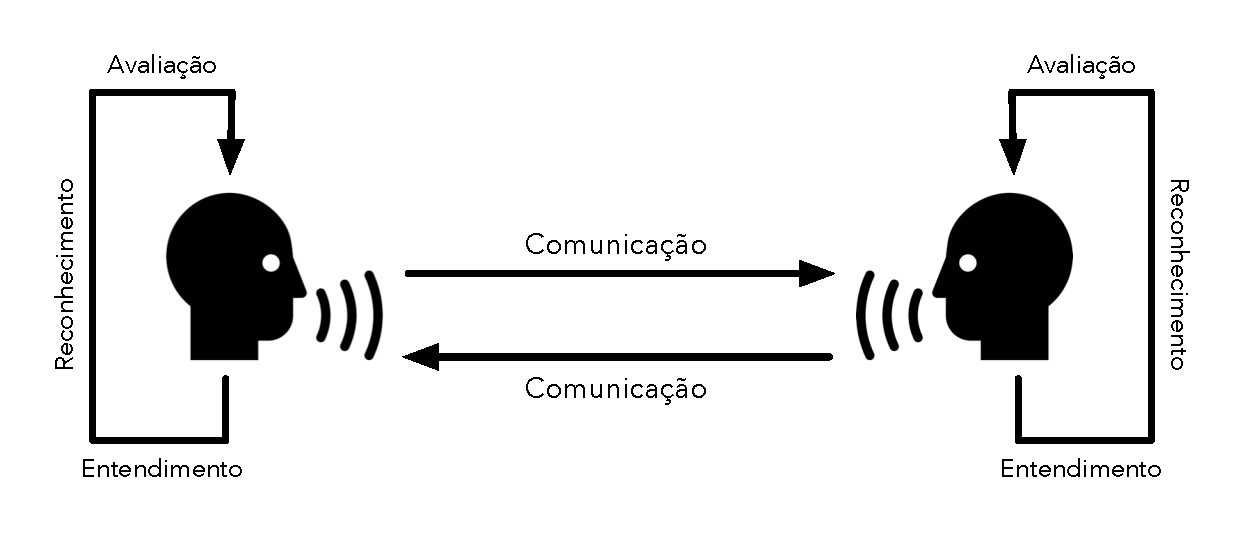
\includegraphics[scale=0.45]{figs/speech_workflow.eps}	
		\label{f.speech_workflow}
		\caption{Processo de comunicação simplificado entre dois seres humanos.}
	\end{figure}
\end{frame}

\begin{frame}
	\begin{itemize}
		\justifying
		\item O objetivo final de um sistema de Processamento de Linguagem Natural é \textbf{compreender e utilizar} uma linguagem da mesma forma que o próprio humano a utiliza;
		\\~\\
		\item Uma compreensão inteligível da linguagem humana requer um \textbf{discernimento} tanto de caracteres como de palavras e, ademais, como ambos estão conectados;
		\\~\\
		\item Enquanto humanos são capazes de aprender e masterizar uma linguagem facilmente, as máquinas ainda esbarram em suas características \textbf{ambíguas} e \textbf{imprecisas}.
	\end{itemize}
\end{frame}

\begin{frame}
	\begin{figure}[!ht]
		\centering
		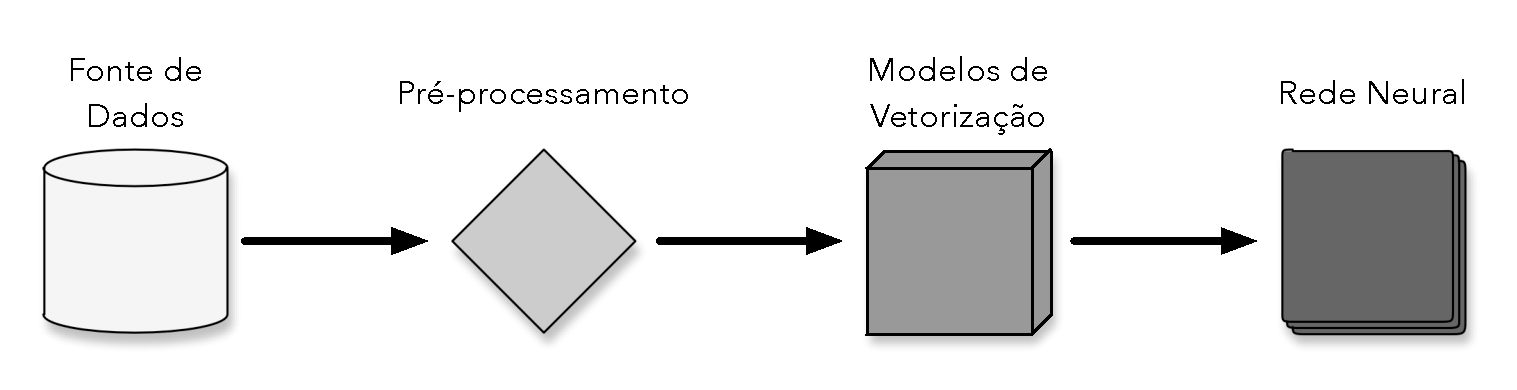
\includegraphics[scale=0.4]{figs/nlp_workflow.eps}	
		\label{f.nlp_workflow}
		\caption{Fluxograma da modelagem de um problema de Processamento de Linguagem Natural.}
	\end{figure}
\end{frame}

\subsection{Exemplos de Tarefas}
\label{ss.tasks}

\begin{frame}{Exemplos de Tarefas}
	\begin{itemize}
		\justifying
		\item Diálogo: Análise de discursos, resolução de correferências e sumarização automática;
		\\~\\
		\item \begin{sloppypar}Semântica: Análise de sentimentos, desambiguação de palavras, entendimento de linguagem natural, extração de relacionamentos, \textbf{geração de linguagem natural}, reconhecimento de entidades nomeadas, reconhecimento de vínculo textual, reconhecimento ótico de caracteres, semântica léxica, semântica distribucional, segmentação de tópicos, sistema de perguntas e respostas e tradução de máquina;	\end{sloppypar}
		\end{itemize}
\end{frame}

\begin{frame}
	\begin{itemize}
		\justifying
		\item Sintaxe: Análise gramatical, extração de terminologias, indução gramatical, lematização, marcação de partes da fala, quebra de sentenças, segmentação de palavras, segmentação morfológica e stemização;
		\\~\\
		\item Voz: conversor de texto para voz, reconhecimento de voz e segmentação de voz.
		\end{itemize}
\end{frame}

\begin{frame}
	\begin{figure}[!ht]
		\centering
		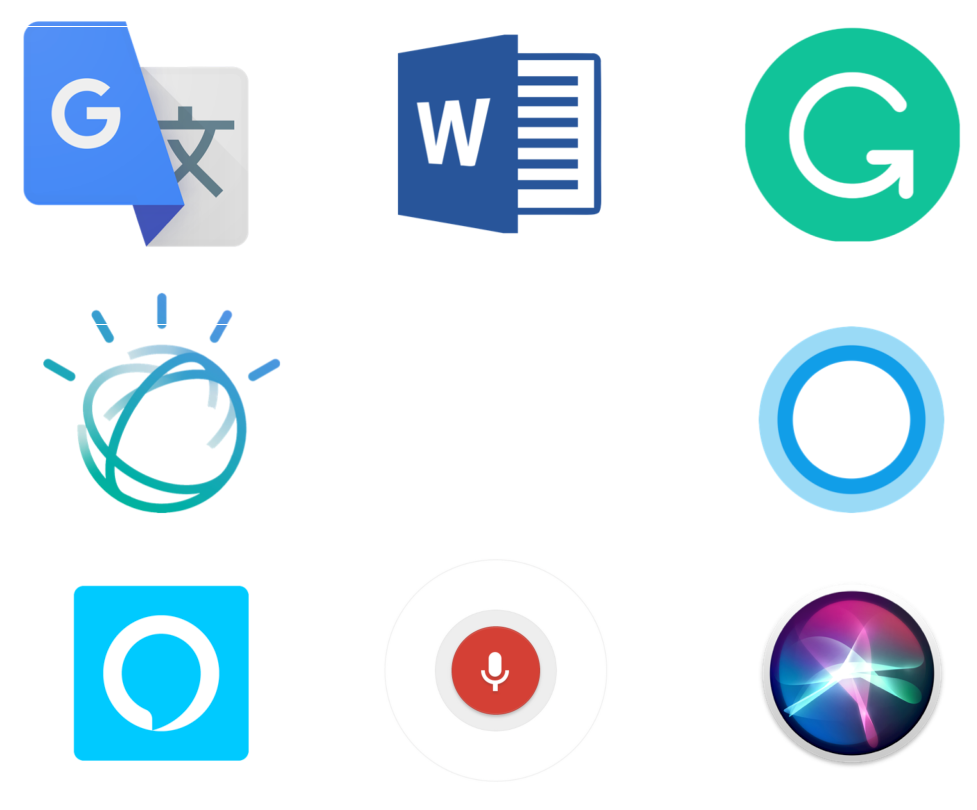
\includegraphics[scale=0.4]{figs/nlp_applications.eps}	
		\label{f.nlp_applications}
		\caption{Exemplos de aplicações baseadas em Processamento de Linguagem Natural. Em sentido horário: \emph{Google Translate}, \emph{Microsoft Word}, \emph{Grammarly}, \emph{Cortana}, \emph{Siri}, \emph{OK Google}, \emph{Alexa} e \emph{IBM Watson}.}
	\end{figure}
\end{frame}

\subsection{Modelagem de Linguagem}
\label{ss.gln}

\begin{frame}{Modelagem de Linguagem}
	\begin{itemize}
		\justifying
		\item A tarefa de modelagem de linguagem refere-se à capacidade de modelos probabilísticos em \textbf{estimar} um $t+1$ estado dado $t$ estados anteriores;
		\\~\\
		\item O modelo linguístico aprende a \textbf{probabilidade de ocorrência} de \emph{tokens} baseado em exemplos;
	\end{itemize}
\end{frame}

\begin{frame}
	\begin{itemize}
		\justifying
		\item O processo de treinamento é baseado em um \textbf{conjunto de exemplos}, não sendo prático para estimar dados não-existentes, por exemplo, \emph{tokens} não encontrados no conjunto de dados;
		\\~\\
		\item Modelos linguísticos são utilizados como \textbf{arquiteturas-base} em tarefas complexas;
		\\~\\
		\item Também podem ser utilizados para a \textbf{geração artificial de texto}.
	\end{itemize}
\end{frame}

\begin{frame}{Geração Artificial de Texto}
	\begin{itemize}
		\justifying
		\item Um modelo linguístico \textbf{adequadamente treinado} é capaz de codificar características e regras do texto em que foi treinado;
		\\~\\
		\item Aprender a \textbf{distribuição probabilística} que representa o conjunto de dados utilizado.
	\end{itemize}
\end{frame}

\begin{frame}
	\begin{itemize}
		\justifying
		\item Distribuição probabilística de um \emph{token} no estado $t$, dado uma sequência prévia de $n$ \emph{tokens}:
		\begin{equation}
			P(w_t | w_{t-1}, w_{t-2}, \ldots, w_{t-n})	
		\end{equation}
		\\~\\
		\item Objetivo é estimar as probabilidades de um \emph{token} $w_{t+1}$ dado uma sequência prévia de $n+1$ \emph{tokens}:
		\begin{equation}
			P(w_{t+1} | w_{t}, w_{t-1}, \ldots, w_{t-n+1})	
		\end{equation}
	\end{itemize}
\end{frame}

\begin{frame}
	\begin{figure}[!ht]
		\centering
		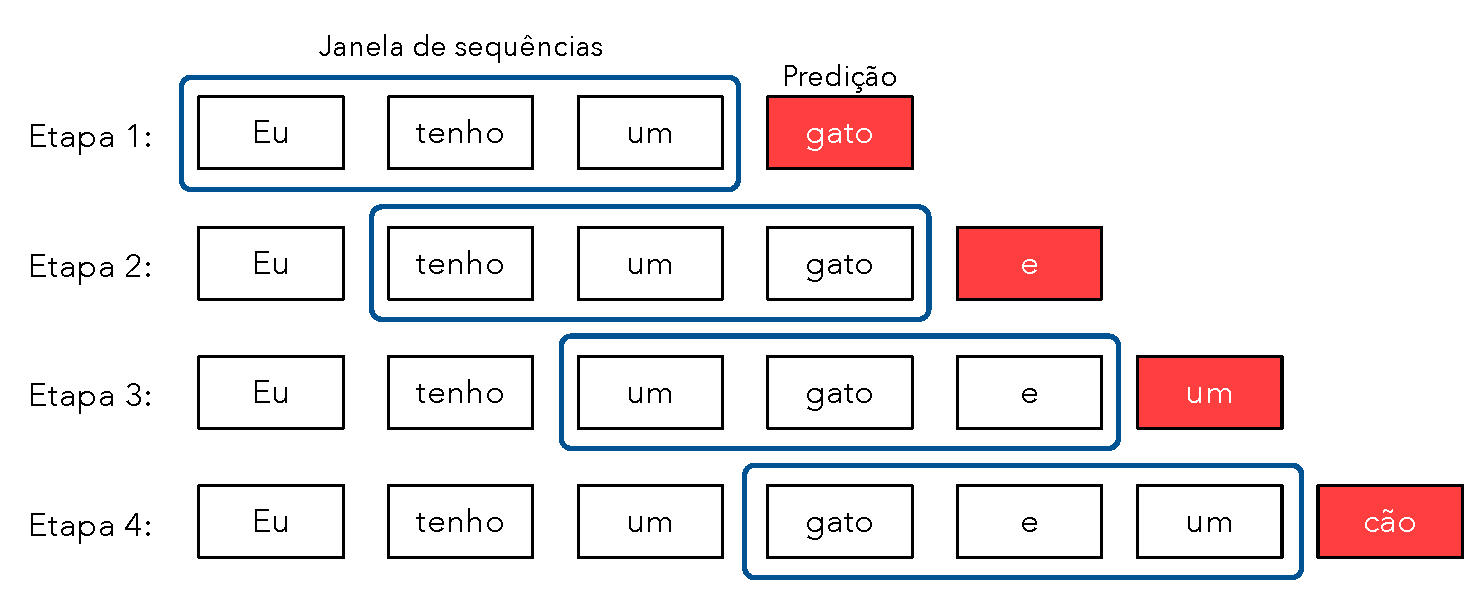
\includegraphics[scale=0.425]{figs/text_generation.eps}	
		\label{f.text_generation}
		\caption{Exemplo de um processo de geração artificial de texto.}
	\end{figure}
\end{frame}